\documentclass[12pt, a4]{article}
\usepackage[english]{babel}
\usepackage[utf8]{inputenc}
\usepackage{fullpage}
\usepackage{listings}
\usepackage{graphicx}
\usepackage{color}

%Syntax highlighting
\definecolor{blue-violet}{rgb}{0.54, 0.17, 0.89}
\definecolor{ao}{rgb}{0.0, 0.5, 0.0}
\definecolor{amaranth}{rgb}{0.9, 0.17, 0.31}
\definecolor{ballblue}{rgb}{0.13, 0.67, 0.8}
\definecolor{onyx}{rgb}{0.06, 0.06, 0.06}


\lstset{
  breaklines=true,                 % automatic line breaking only at whitespace
  captionpos=b,                    % sets the caption-position to bottom
  breakatwhitespace=false,
  keepspaces=true,
  numbers=left,
  numbersep=5pt,
  showspaces=false,
  showstringspaces=false,
  showtabs=false,
  tabsize=4,  
  backgroundcolor=\color{white},   % choose the background color
  commentstyle=\color{ao},    % comment style
  keywordstyle=\color{amaranth},    % keyword style
  stringstyle=\color{blue-violet},    % string literal style
  numberstyle=\tiny\color{ballblue},	   % number style
  basicstyle=\ttfamily\footnotesize\color{onyx} % size of fonts used for the code
}


%Document Header
\title{\textbf{Department of CSE\\SSN College of Engineering}}
\author{\textbf{Vishakan Subramanian - 18 5001 196 - Semester VI}}
\date{20 April 2021}

\begin{document}
\maketitle
\hrule
\section*{\center{UCS 1611 - Internet Programming Lab}}
\hrule
\bigskip

%Assignment Details
\subsection*{\center{\textbf{Exercise 7: Website for International Conference using React}}}
\subsection*{\flushleft{Learning Objective:}}
\begin{flushleft}
Design a Website for an International Conference using React. (Similar to Ex 1)

\begin{enumerate}
\item The conference homepage should consists of the following tabs:
Home, Committee, Call For Papers, Important Dates, Workshops,
Registration and Contact.
\item On clicking each tab, it should open in the same page (SPA). (Use react
router)
\item The website should contain logos, header, footer.
\item The Header and footer should be same for all links.
\item For pre-conference workshop registration use form elements.
\end{enumerate}
 
\end{flushleft}

%Code
\newpage
\subsection*{\flushleft{Code - Home Component:}}
\begin{flushleft}
\lstinputlisting[language = HTML]{conference/src/components/Home.js}
\end{flushleft}

\newpage
\subsection*{\flushleft{Code - Committee Component:}}
\begin{flushleft}
\lstinputlisting[language = HTML]{conference/src/components/Committee.js}
\end{flushleft}

\newpage
\subsection*{\flushleft{Code - Call for Papers Component:}}
\begin{flushleft}
\lstinputlisting[language = HTML]{conference/src/components/Papers.js}
\end{flushleft}

\newpage
\subsection*{\flushleft{Code - Important Dates Component:}}
\begin{flushleft}
\lstinputlisting[language = HTML]{conference/src/components/Dates.js}
\end{flushleft}

\newpage
\subsection*{\flushleft{Code - Workshops Component:}}
\begin{flushleft}
\lstinputlisting[language = HTML]{conference/src/components/Workshops.js}
\end{flushleft}

\newpage
\subsection*{\flushleft{Code - Registration Component:}}
\begin{flushleft}
\lstinputlisting[language = HTML]{conference/src/components/Registration.js}
\end{flushleft}

\newpage
\subsection*{\flushleft{Code - Contact Component:}}
\begin{flushleft}
\lstinputlisting[language = HTML]{conference/src/components/Contact.js}
\end{flushleft}

\newpage
\subsection*{\flushleft{Code - Header Component:}}
\begin{flushleft}
\lstinputlisting[language = HTML]{conference/src/components/Header.js}
\end{flushleft}

\newpage
\subsection*{\flushleft{Code - Footer Component:}}
\begin{flushleft}
\lstinputlisting[language = HTML]{conference/src/components/Footer.js}
\end{flushleft}

\newpage
\subsection*{\flushleft{Code - App JS:}}
\begin{flushleft}
\lstinputlisting[language = HTML]{conference/src/App.js}
\end{flushleft}



\newpage
\subsection*{\flushleft{Code - Stylesheet:}}
\begin{flushleft}
\lstinputlisting[]{conference/src/styles.css}
\end{flushleft}

%Output
\newpage
\subsection*{\flushleft{Output - Home Page:}}
\begin{figure}[h]
\centering
\caption{Browser Output: Home Page.}
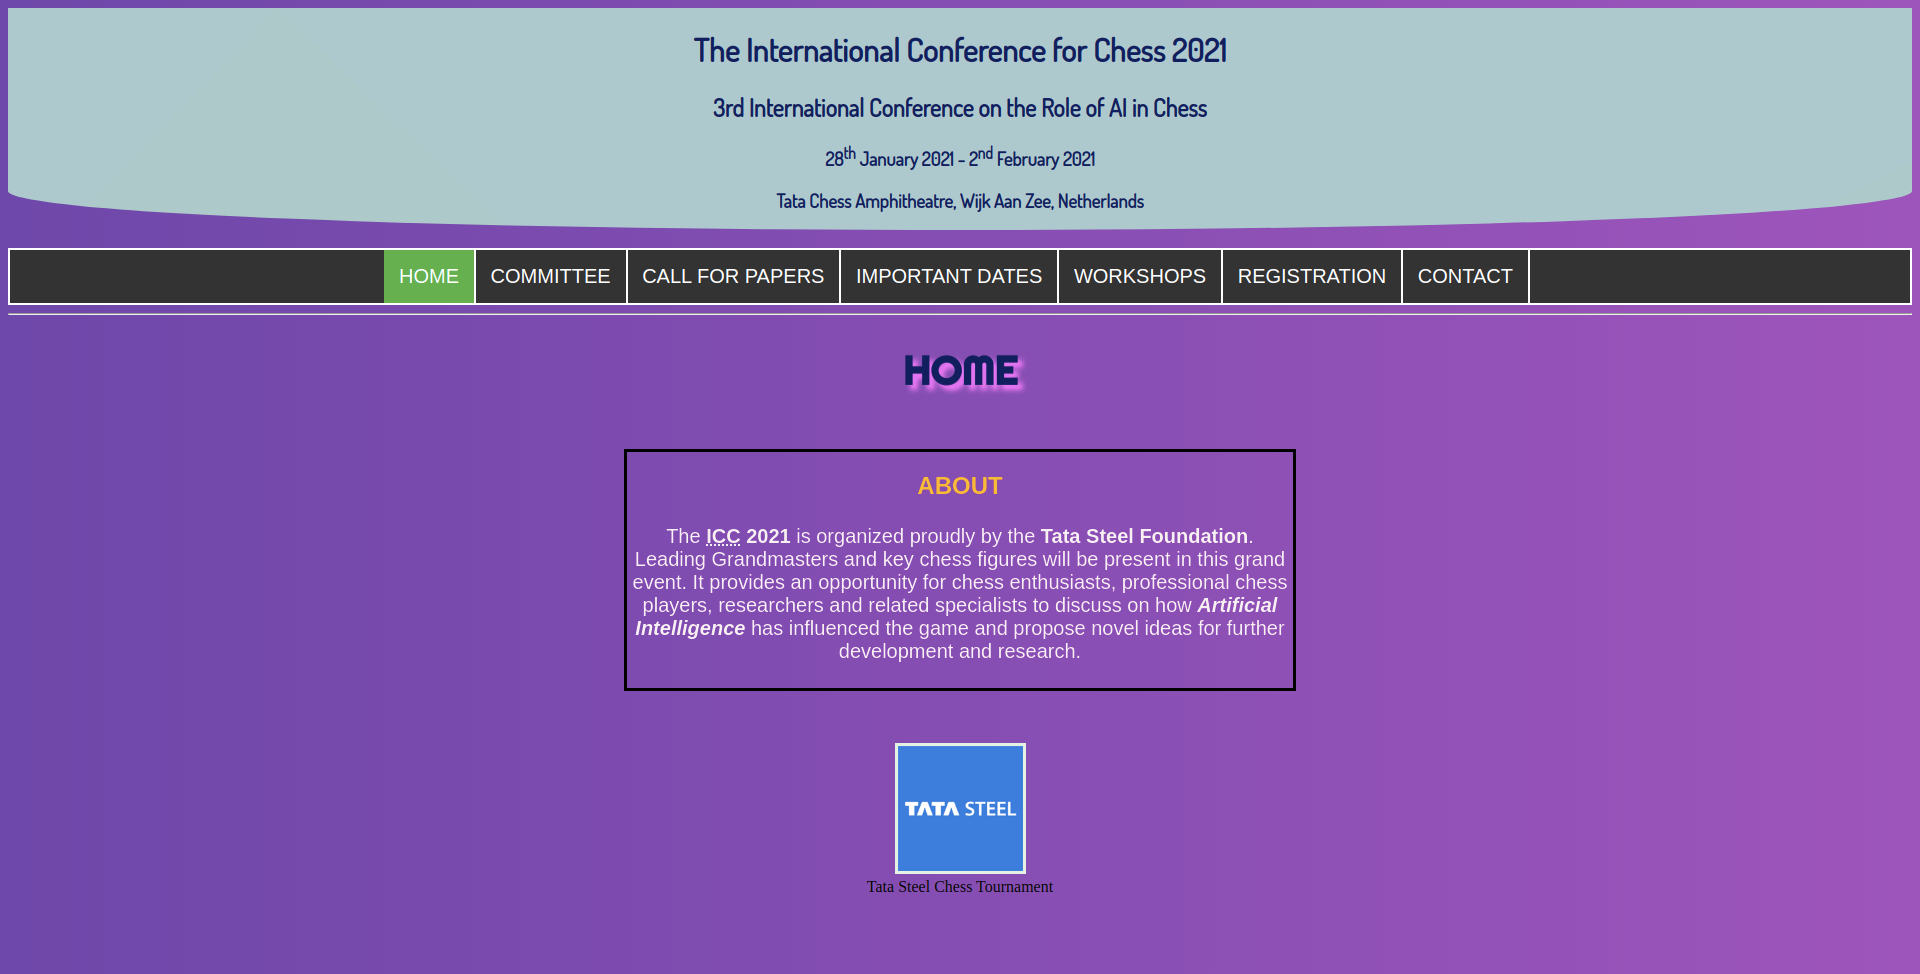
\includegraphics[height=10cm, width=18cm, keepaspectratio]{Output/Home.png}
\end{figure}

\newpage
\subsection*{\flushleft{Output - Committee Page:}}
\begin{figure}[h]
\centering
\caption{Browser Output: Committee Page.}
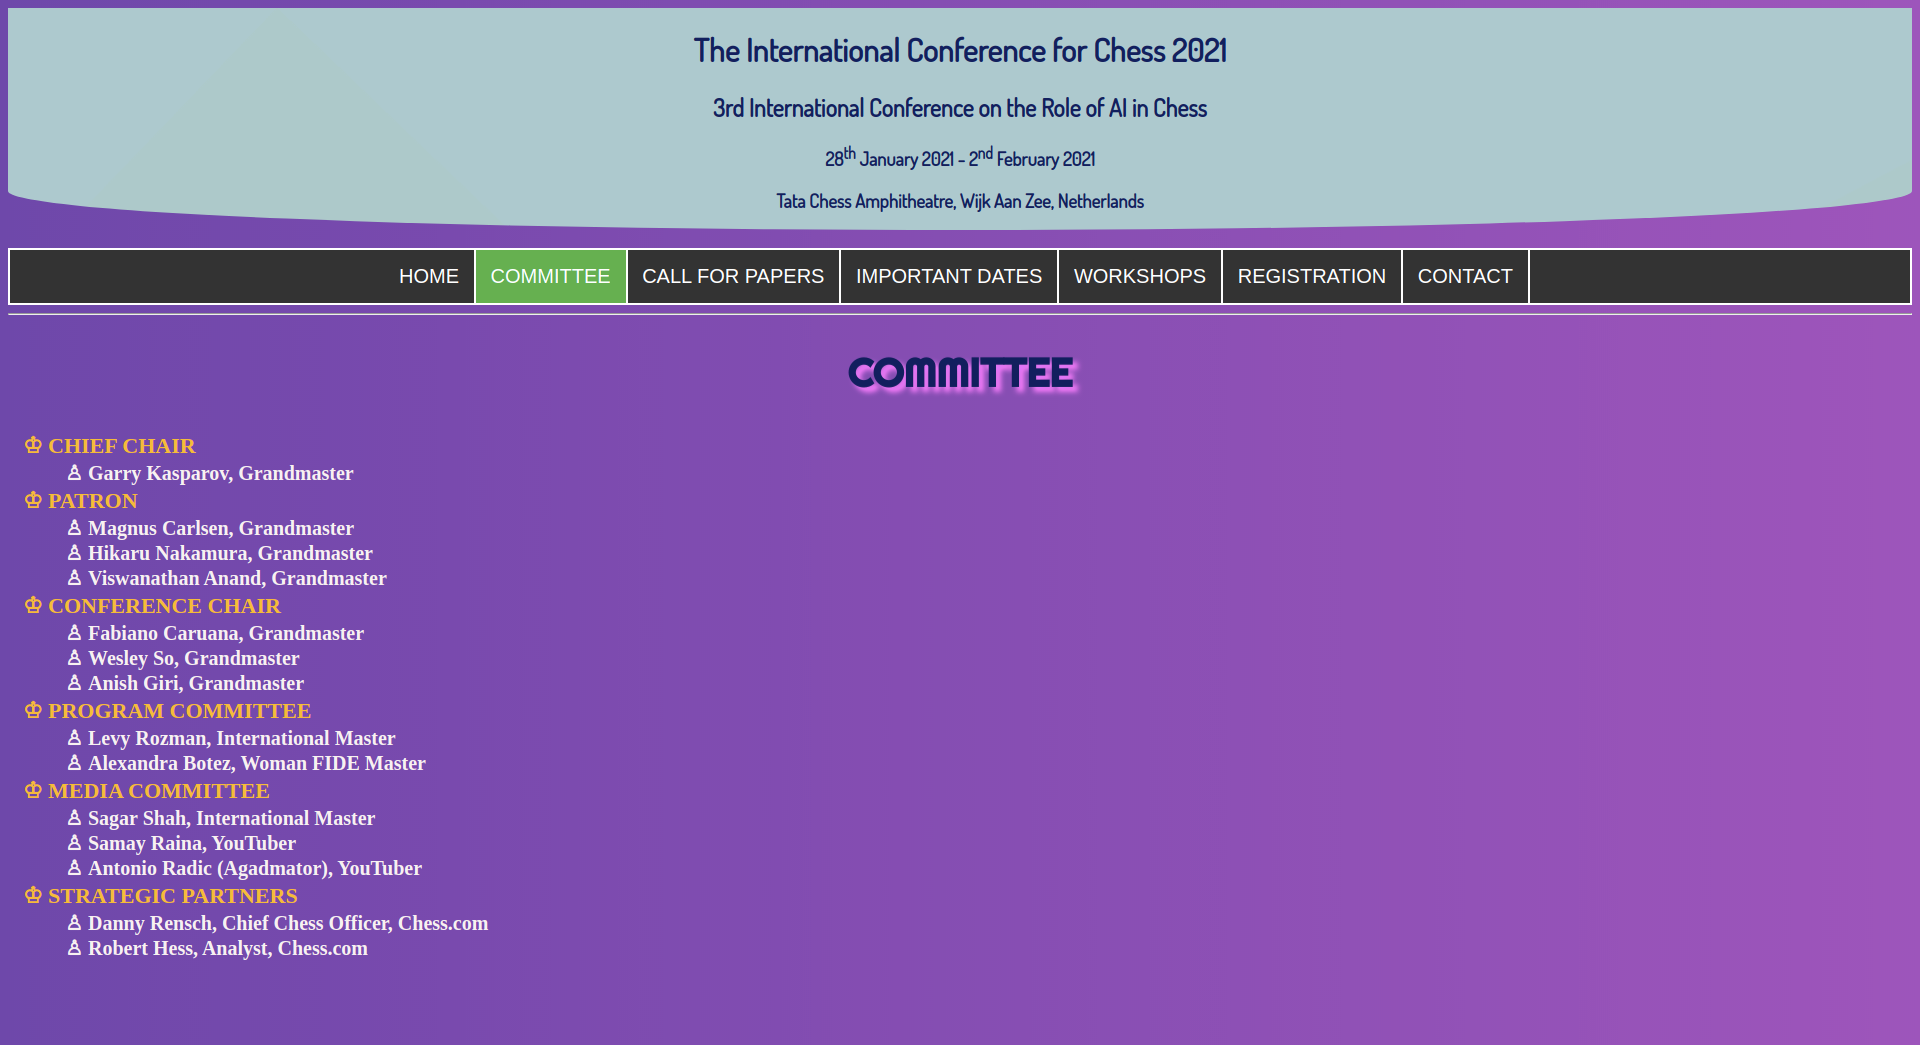
\includegraphics[height=10cm, width=18cm, keepaspectratio]{Output/Committee.png}
\end{figure}

\newpage
\subsection*{\flushleft{Output - Call For Papers Page:}}
\begin{figure}[h]
\centering
\caption{Browser Output: Call For Papers Page.}
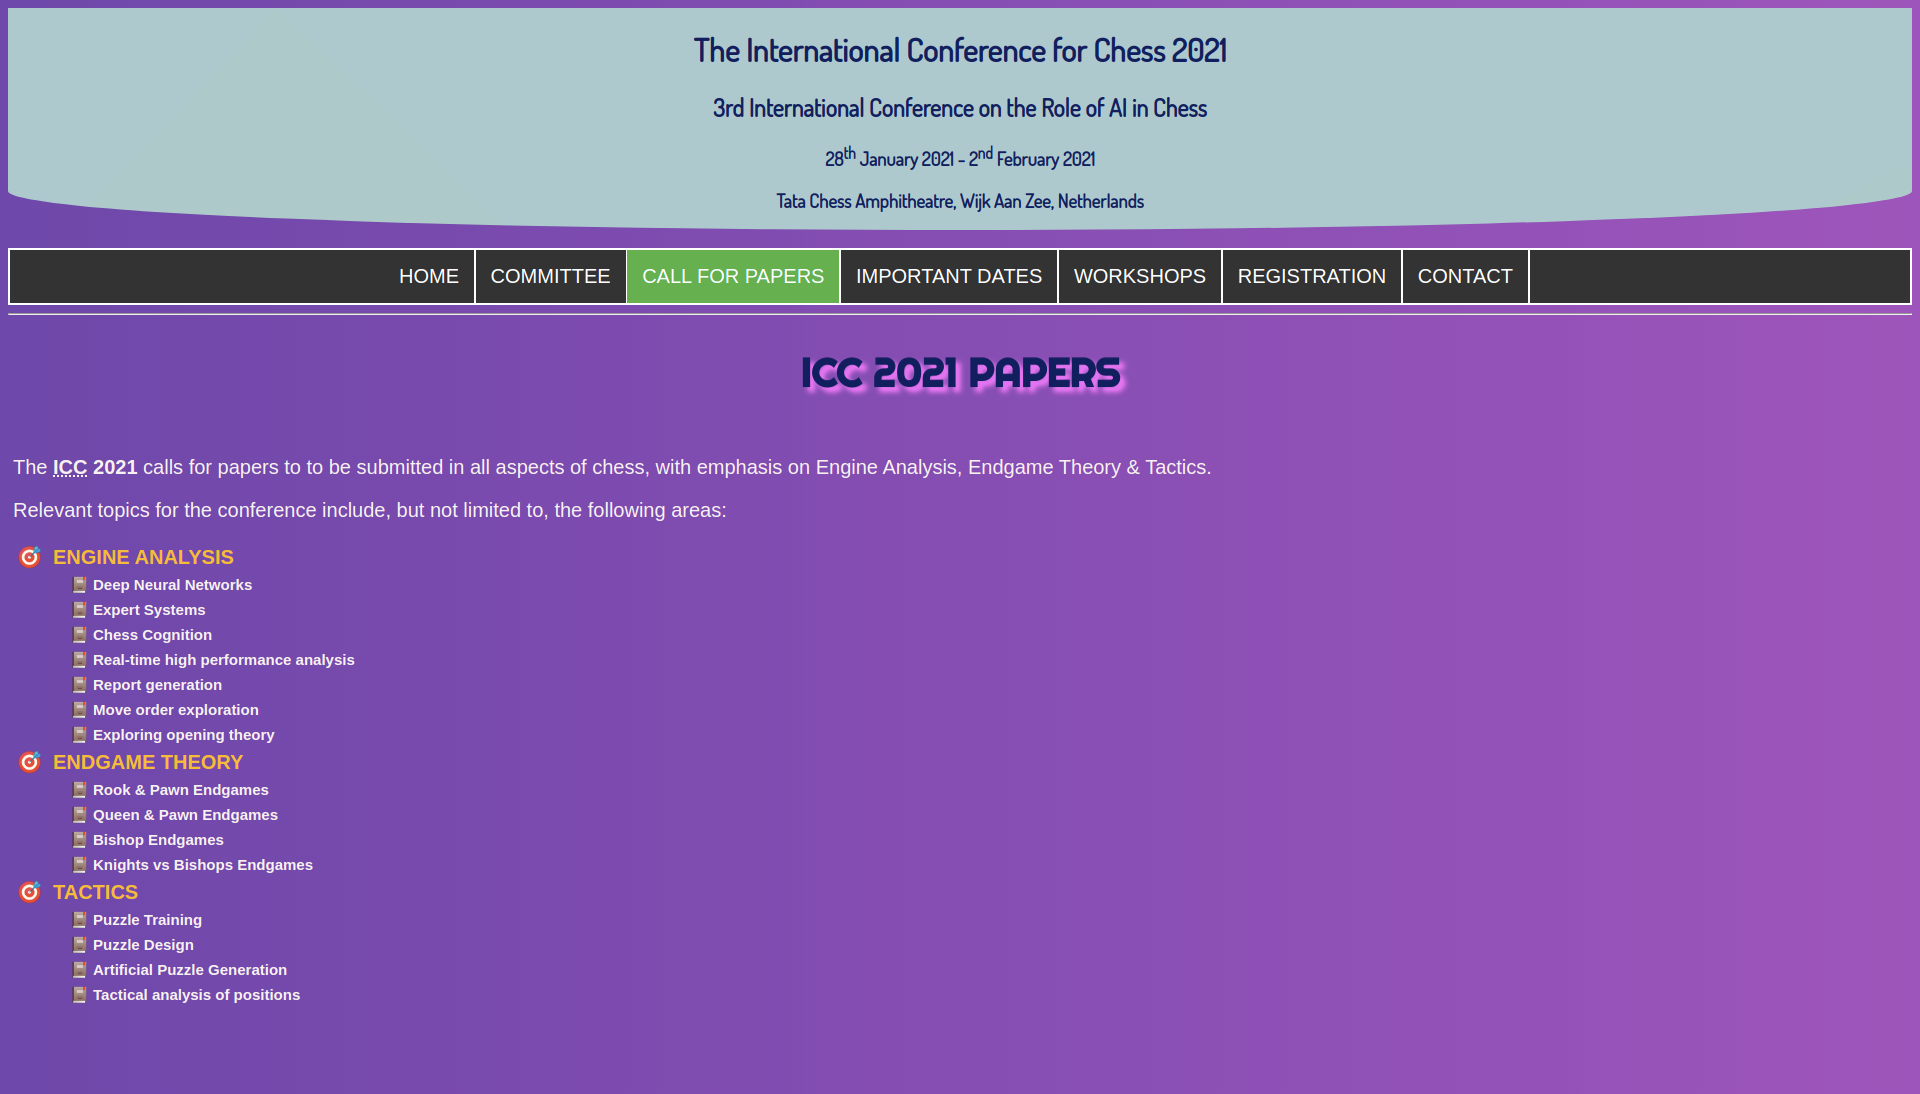
\includegraphics[height=10cm, width=18cm, keepaspectratio]{Output/Papers.png}
\end{figure}

\newpage
\subsection*{\flushleft{Output - Important Dates Page:}}
\begin{figure}[h]
\centering
\caption{Browser Output: Important Dates Page.}
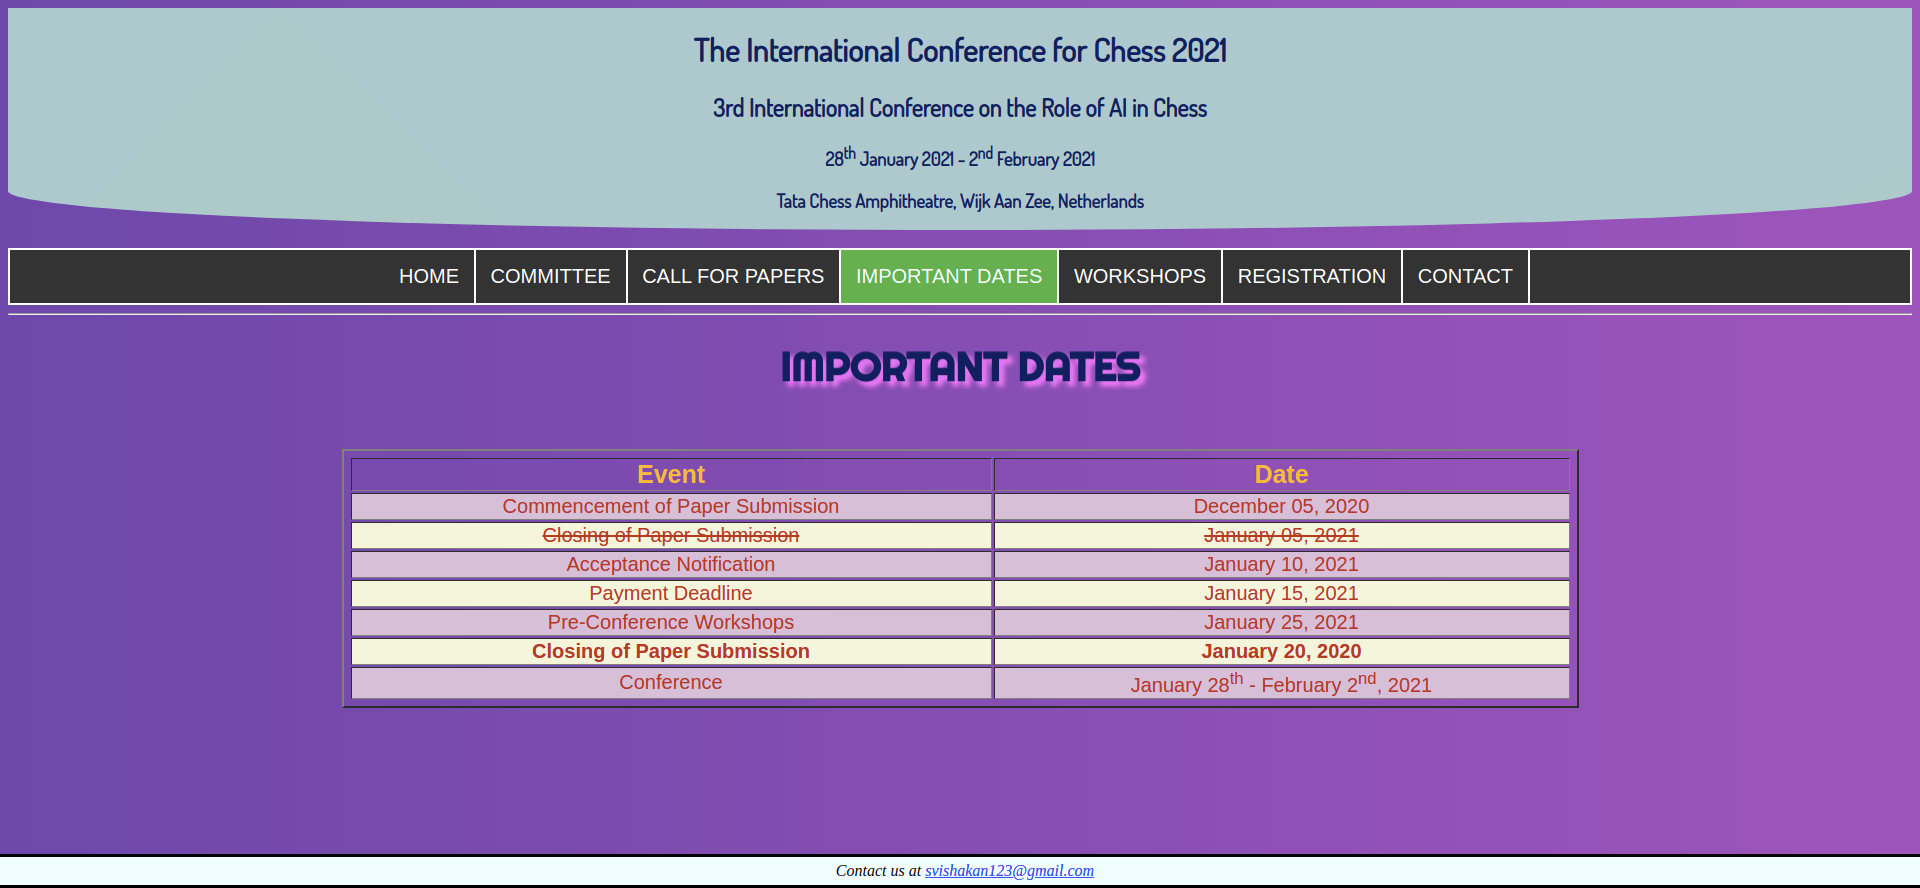
\includegraphics[height=10cm, width=18cm, keepaspectratio]{Output/Dates.png}
\end{figure}

\newpage
\subsection*{\flushleft{Output - Workshops Page:}}
\begin{figure}[h]
\centering
\caption{Browser Output: Workshops Page.}
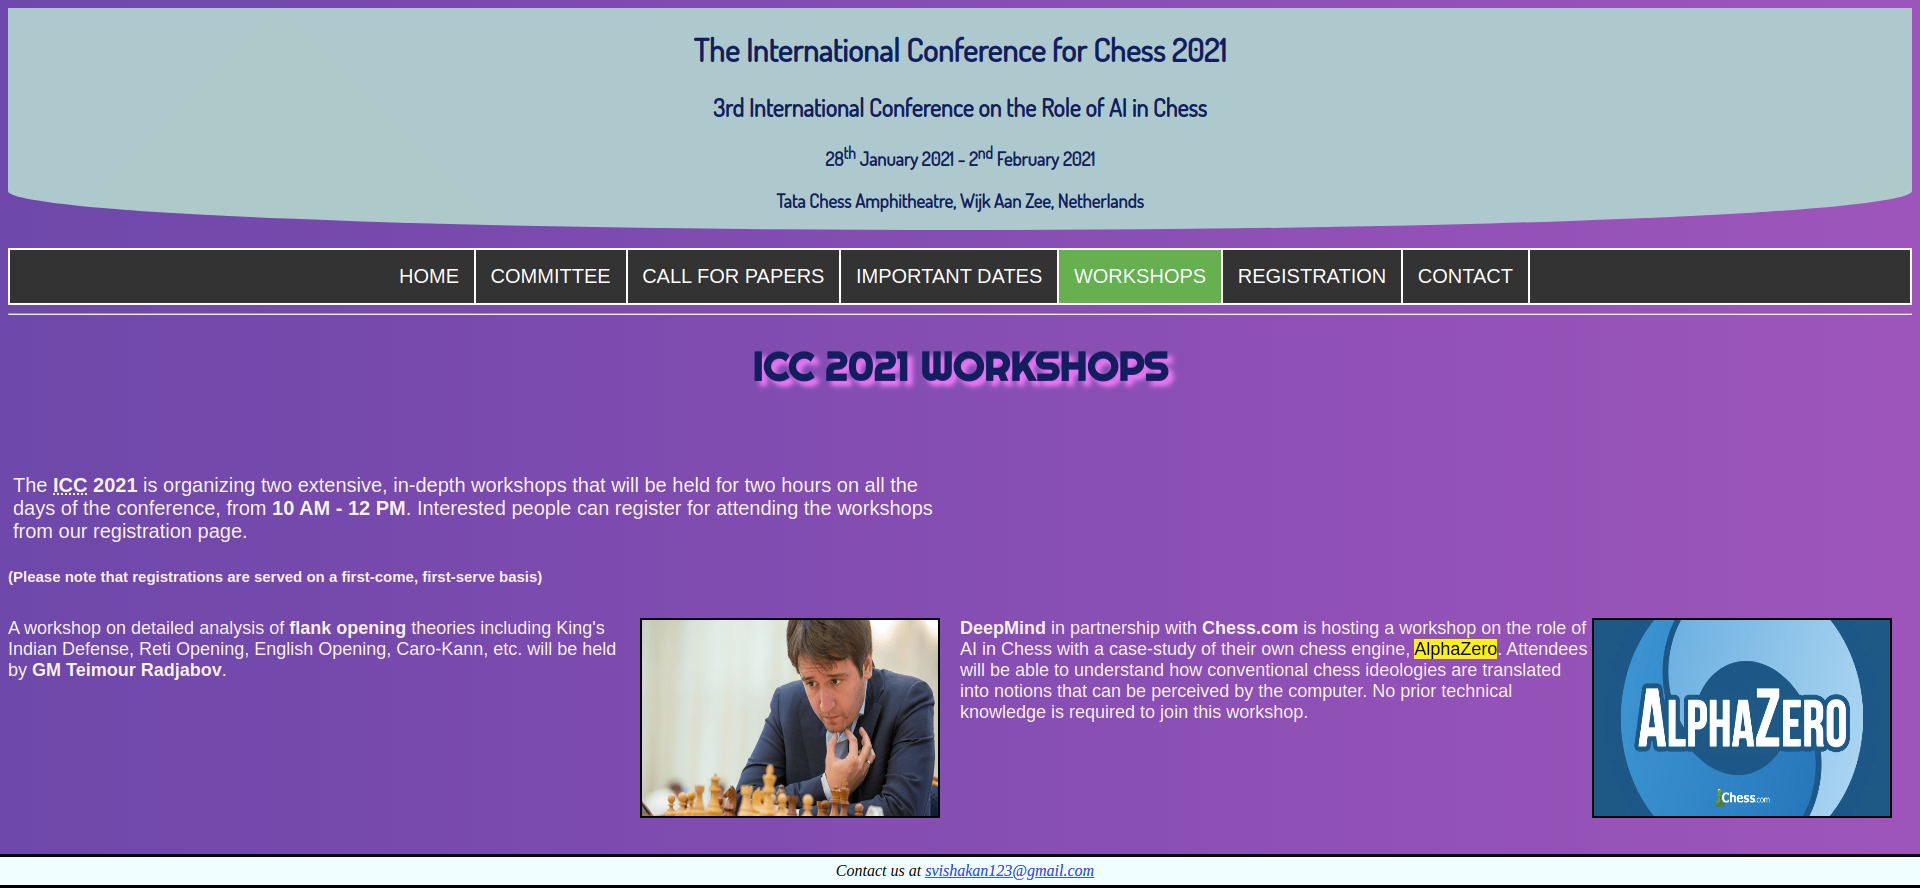
\includegraphics[height=10cm, width=18cm, keepaspectratio]{Output/Workshops.png}
\end{figure}

\newpage
\subsection*{\flushleft{Output - Registration Page:}}
\begin{figure}[h]
\centering
\caption{Browser Output: Registration Page.}
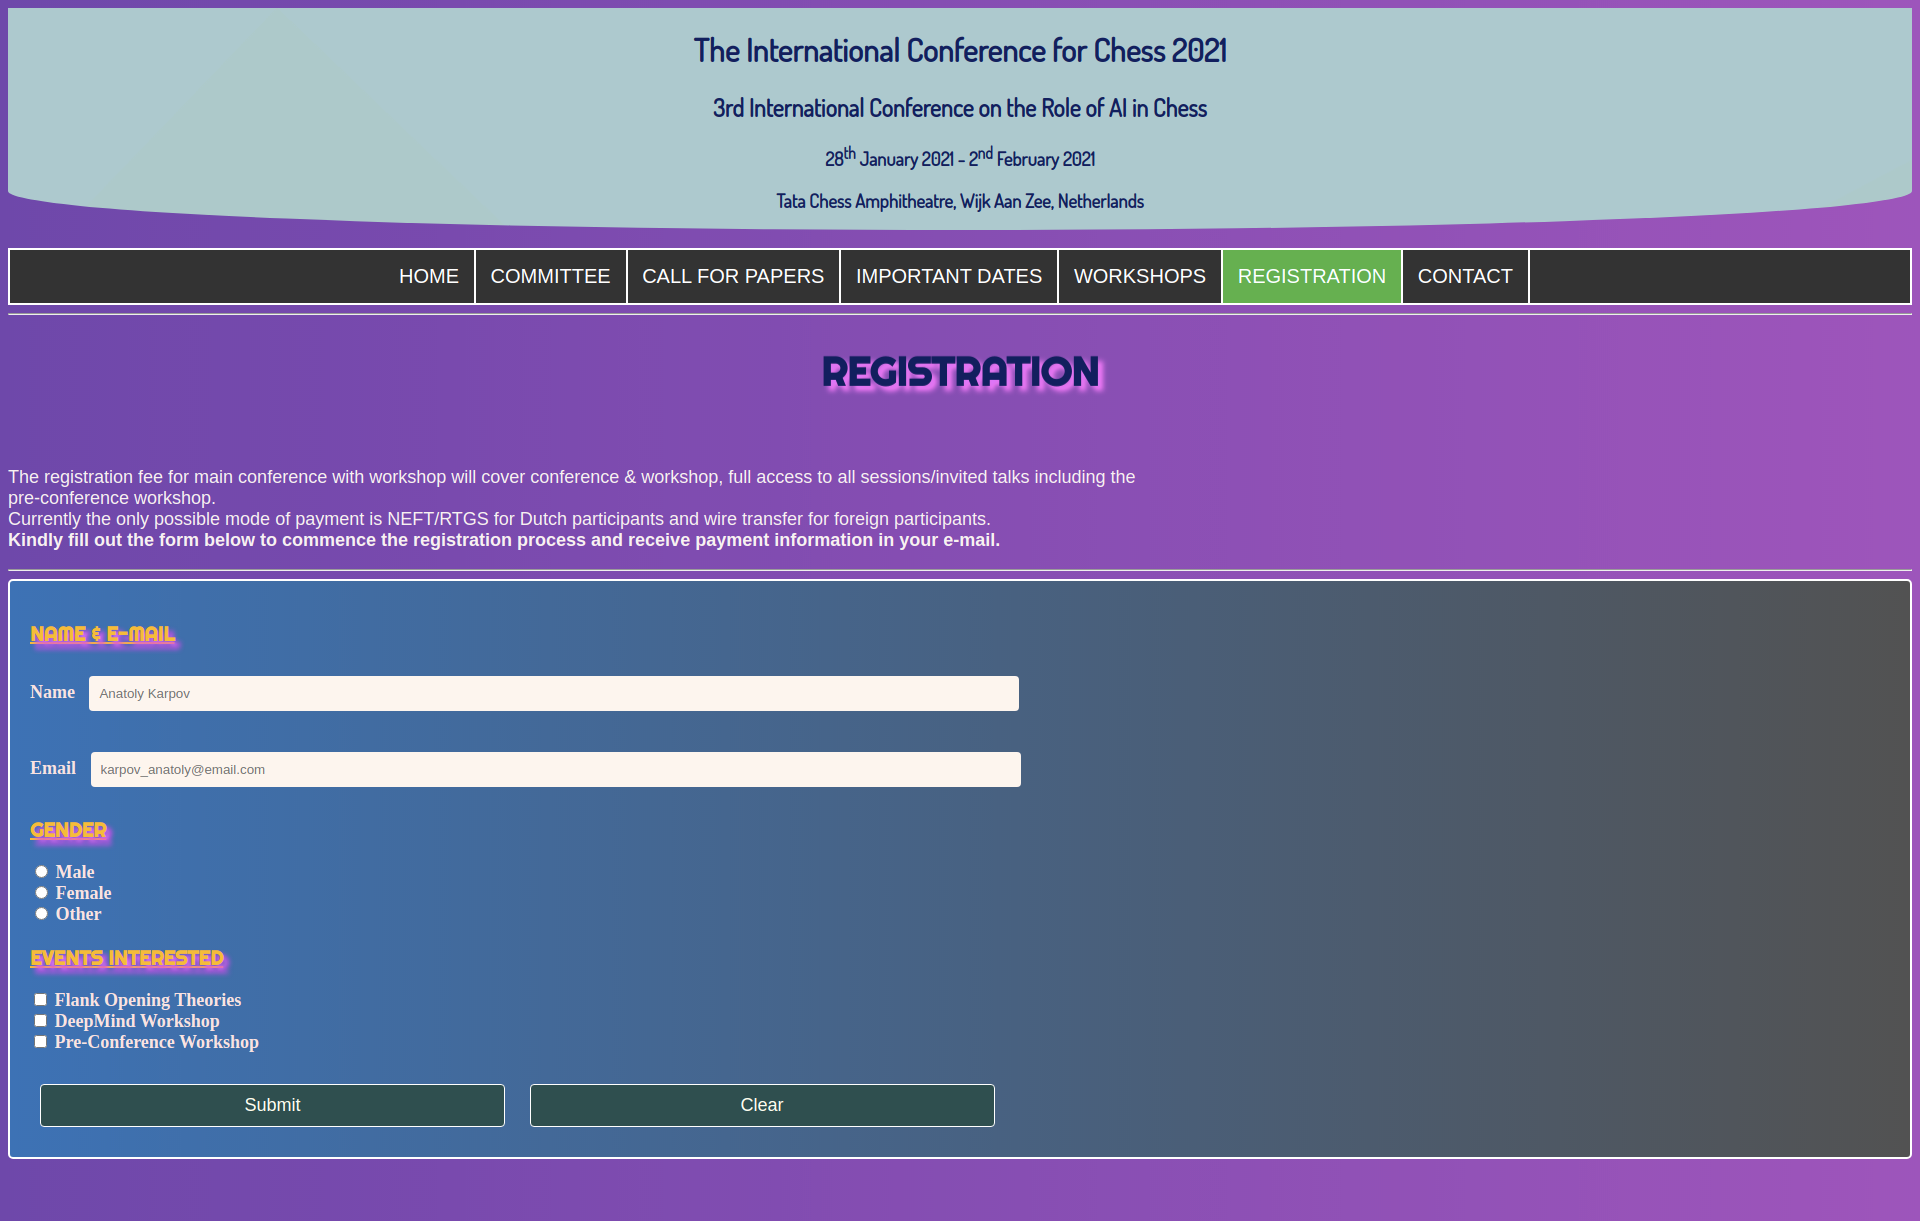
\includegraphics[height=10cm, width=18cm, keepaspectratio]{Output/Reg.png}
\end{figure}


\newpage
\subsection*{\flushleft{Output - Contact Page:}}
\begin{figure}[h]
\centering
\caption{Browser Output: Contact Page.}
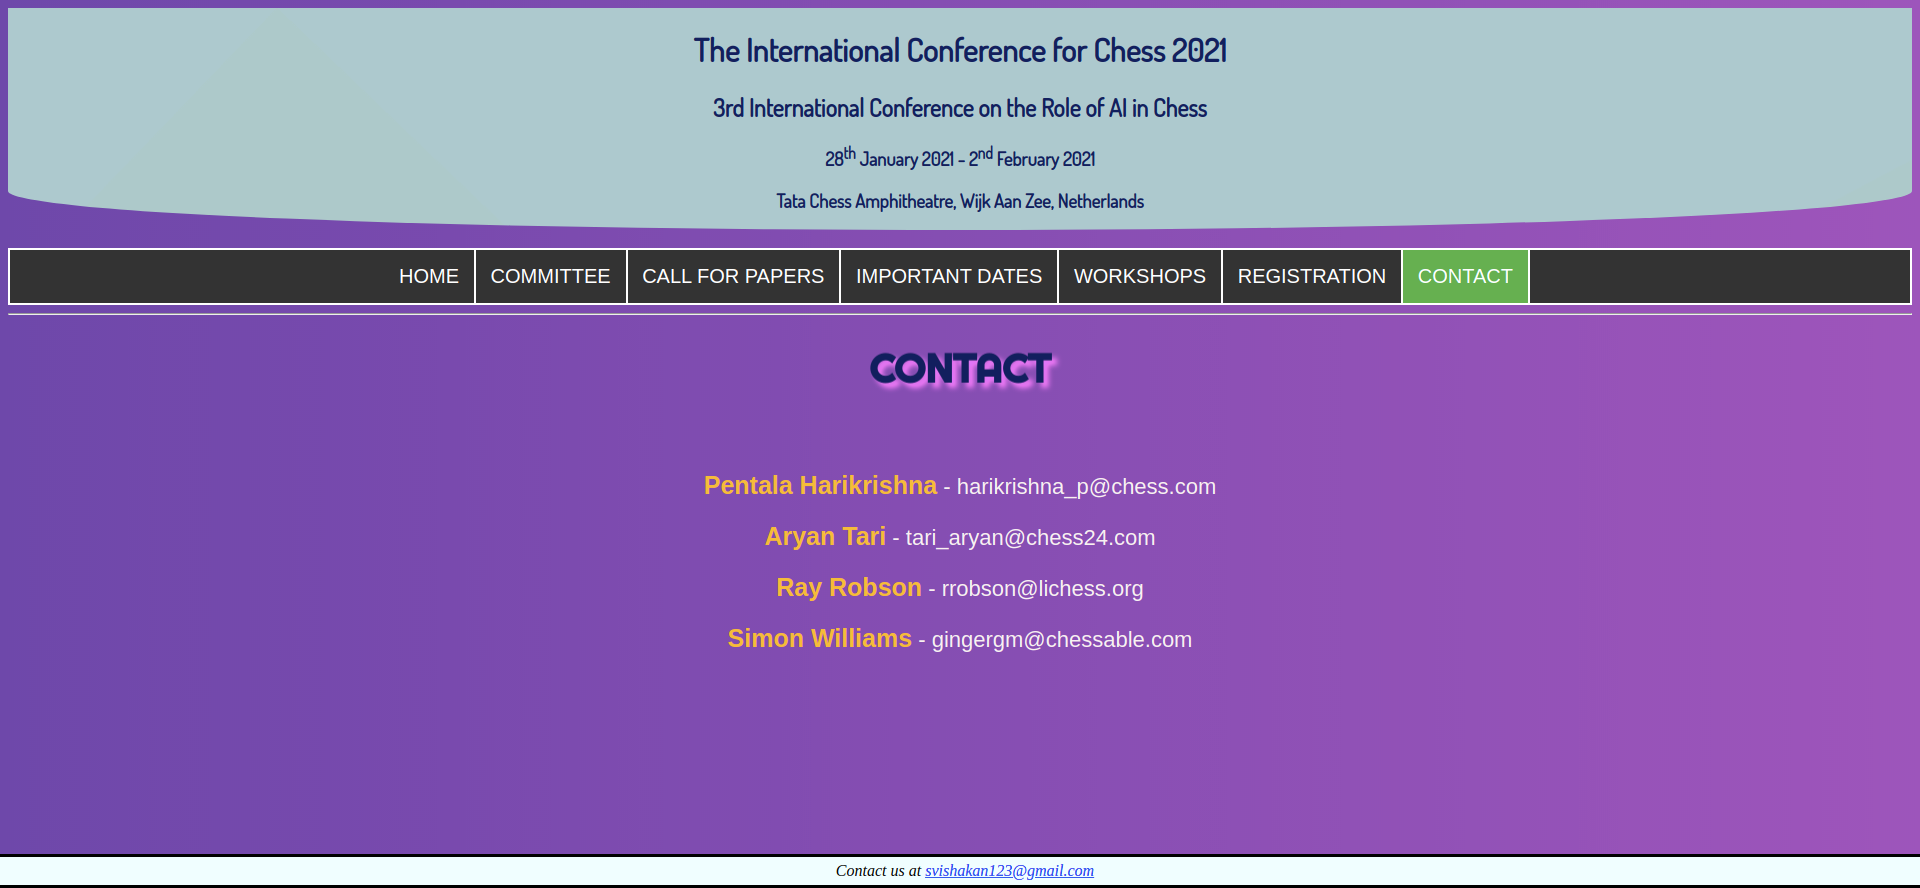
\includegraphics[height=10cm, width=18cm, keepaspectratio]{Output/Contact.png}
\end{figure}

%Learning Outcome
\newpage
\subsection*{\flushleft{Learning Outcome:}}
\begin{itemize}

\item From the experiment, I learnt to create a simple \textbf{React} app.
\item I learnt to create and render a class component.
\item I learnt to create a SPA with multiple links in React.
\item I learnt about the working of \textbf{React Router}.
\item I was able to reuse my previous HTML elements and convert them to JSX format for rendering in React.
\item I learnt how components are rendered in React.
\item I learnt about JSX syntax.
\item I learnt how to load different components based on user-selection using React Routing.
\item I was able to modularize and reuse several components like the header, navigation bar and footer using React.
\item I learnt how to download different NodeJS packages.
\item I implemented detailed CSS for the website.
\item I learnt how react efficiently simplifies code using the principle of reuse.

\end{itemize}

\end{document}
